\paragraph{QuizziPedia::Front-End::Directives::EliminationAndModifyDirective}
\begin{figure} [ht]
	\centering
	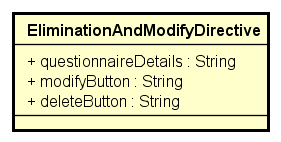
\includegraphics[scale=0.80]{UML/Classi/Front-End/QuizziPedia_Front-end_EliminationAndModifyDirective.png}
	\caption{QuizziPedia::Front-End::Views:EliminationAndModifyDirective}
\end{figure} \FloatBarrier
\begin{itemize}
	\item \textbf{Descrizione}: componente grafico contenente i bottoni per eliminare o modificare un questionario;
	\item \textbf{Utilizzo}: permette di eliminare un questionario o di modificarne uno esistente;
	\item \textbf{Relazioni con altre classi}:
	\begin{itemize}
		\item \textit{IN} \texttt{QuizEventController}: questa classe permette di reagire ai comandi dell'utente durante la gestione dei suoi questionari;
		\item \textit{IN} \texttt{LangModel}: rappresenta il modello delle informazioni per la giusta traduzione dell'applicazione;
		\item \textit{IN} \texttt{QuizEventModelView}: classe di tipo modelview la cui istanziazione è contenuta all'interno della variabile di ambiente \$scope di \textit{Angular.js\ped{G}}. All'interno di essa sono presenti le variabili e i metodi necessari per il \textit{Two-Way Data-Binding\ped{G}} tra le directive \texttt{EliminationAndModifyDirective}, \texttt{ExamModalityDirective} e \texttt{QuestionnaireResultsDirective} e il controller \texttt{QuizEventController};
		\item \textit{OUT} \texttt{QuestionnaireManagementView}: view principale per la gestione dei questionari.
	\end{itemize}
	\item \textbf{Attributi}:
	\begin{itemize}
		\item \texttt{+ modifyButtonElimination: String} \\ Attributo che viene utilizzato per visualizzare la giusta traduzione della \textit{label\ped{G}} per il bottone di modifica del questionario selezionato, in italiano o in inglese; 
		\item \texttt{+ deleteButtonElimination: String} \\ Attributo che viene utilizzato per visualizzare la giusta traduzione della \textit{label\ped{G}} per il bottone di eliminazione del questionario selezionato, in italiano o in inglese;
		\item \texttt{+ controller: String} \\ Stringa contenente il nome del controller della direttiva;
		\item \texttt{+ restrict: String} \\ Stringa che permette di definire le modalità di inserimento della direttiva all'interno della pagina;
		\item \texttt{+ scope: Scope} \\ Oggetto scope interno della direttiva, contiene le funzionalità per gestire i dati presenti all'interno;
		\item \texttt{+ templateUrl: String} \\ Stringa contenente il percorso del file \textit{HTML\ped{G}} che contiene la direttive.
	\end{itemize}
\end{itemize}